\section{Sensor Interrogation Principle}
Lecture 12 introduces the general idea that optical sensors can be interrogated by converting an optical wavelength, phase, time, position, frequency, or amplitude change into an electrical readout \cite{lecture12a}. For microring resonator sensors, the most direct readout is spectral: a perturbation changes the effective index and therefore moves the resonance wavelength. This can be expressed qualitatively as
\begin{equation}
\Delta n_{\mathrm{eff}} \rightarrow \Delta \lambda_{\mathrm{res}} .
\end{equation}

Relevant interrogation methods include wavelength scanning interrogation, fixed-wavelength intensity interrogation, resonance tracking, and spectral shift measurement. In wavelength scanning, a tunable source or optical spectrum analyser maps the resonance peak or notch directly. In fixed-wavelength intensity interrogation, the laser is biased on the slope of a resonance and a wavelength shift is converted into an intensity change. Resonance tracking uses feedback to keep the laser or filter locked to the resonance. Spectral interrogation is robust and physically transparent, but its resolution depends on wavelength sampling, source stability, detector noise, thermal drift, and resonance linewidth.

Lecture 12 B connects these principles to integrated optic sensors, including SOI microring sensors and amplitude-comparison schemes using through and drop ports \cite{lecture12b}. The same core idea applies here: analyte binding or an environmental perturbation changes the ring optical path length, causing a measurable resonance shift.

\begin{figure}[H]
\centering
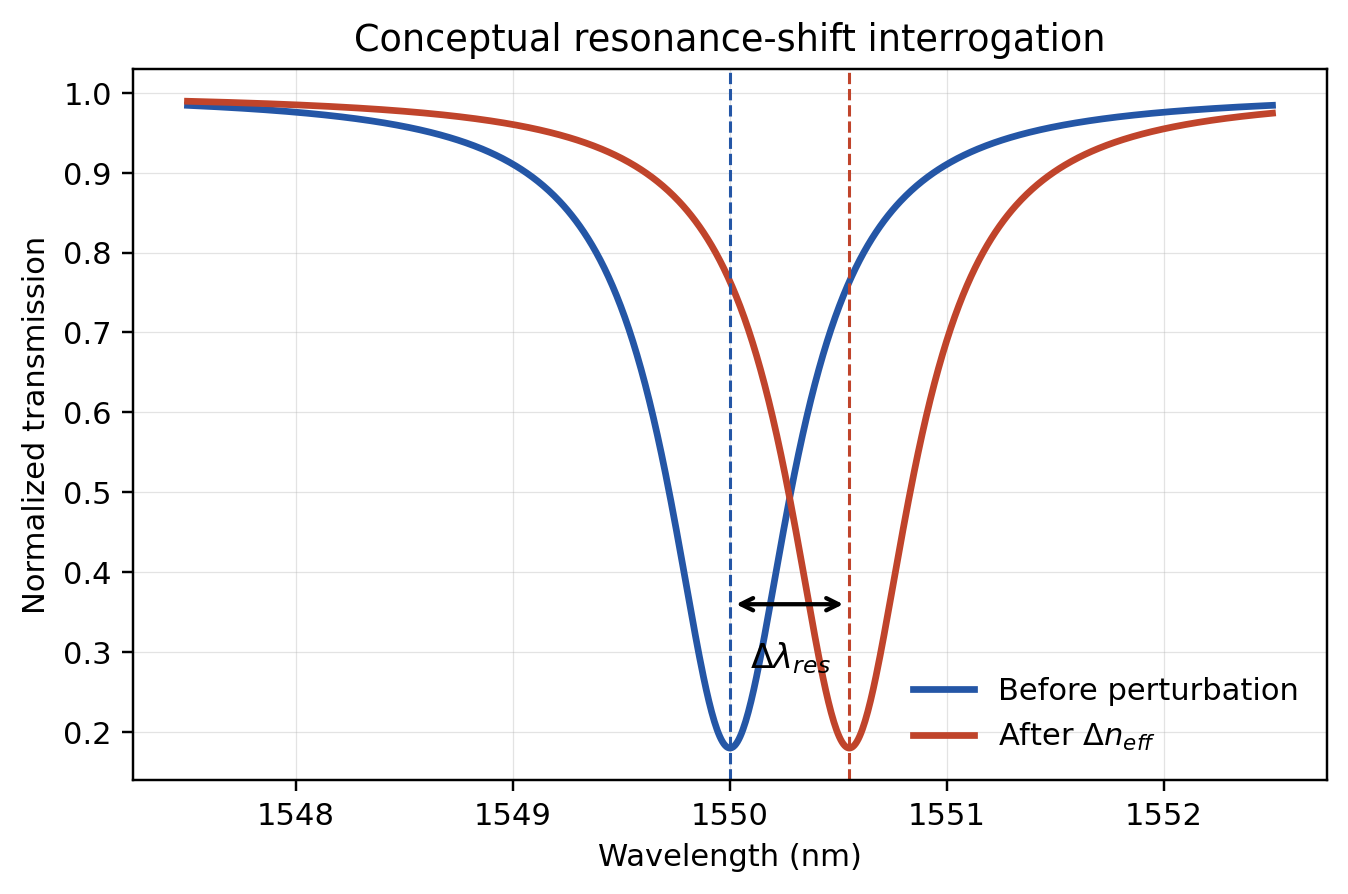
\includegraphics[width=0.78\linewidth]{figures/interrogation_principle_schematic.png}
\caption{Conceptual spectral interrogation of a microring resonance. The plot illustrates the expected direction of a resonance shift under a change in \(n_{\mathrm{eff}}\); it is not a simulated spectrum.}
\label{fig:interrogation}
\end{figure}

\section{Microring Resonator Theory}
An add-drop microring contains two straight bus waveguides and a ring waveguide, as shown in Fig.~\ref{fig:ring-schematic}. Light is coupled into the ring through evanescent coupling. At resonance, constructive interference builds the circulating field, producing a drop-port response and a through-port notch.

\begin{figure}[H]
\centering
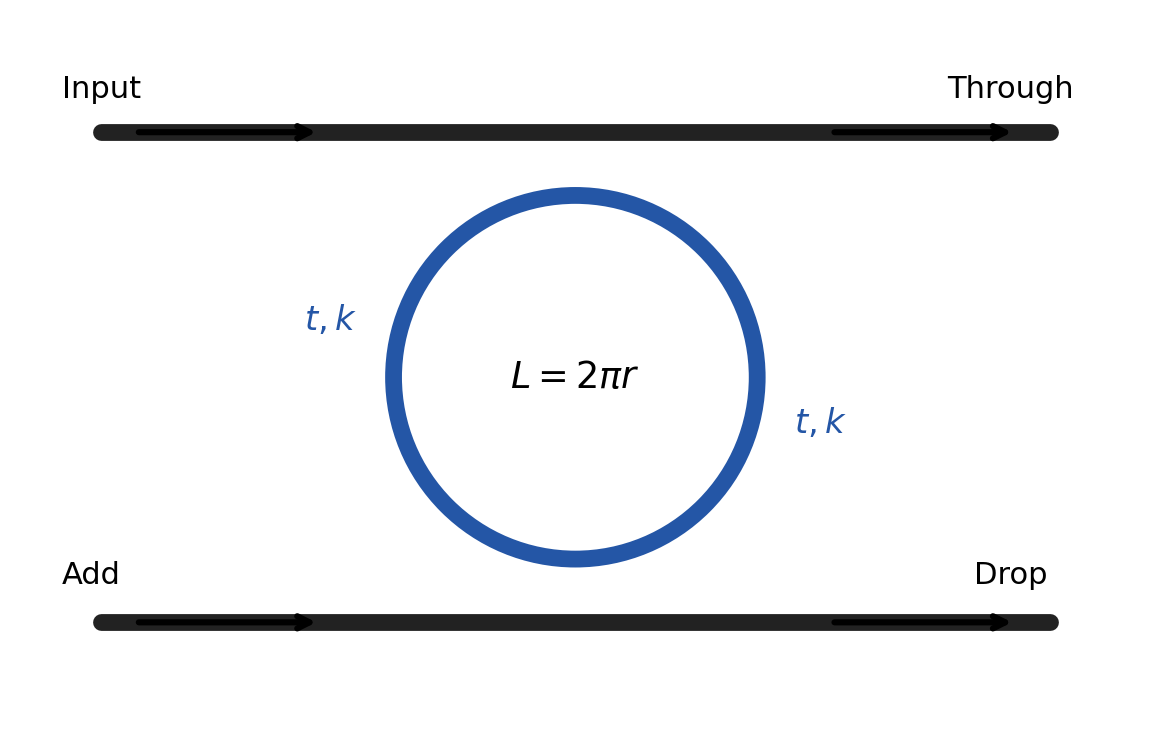
\includegraphics[width=0.76\linewidth]{figures/microring_add_drop_schematic.png}
\caption{Conceptual add-drop microring resonator. The field coupling coefficients are represented by through amplitude \(t\) and cross-coupling amplitude \(k\).}
\label{fig:ring-schematic}
\end{figure}

The resonance condition is
\begin{equation}
N \lambda_{\mathrm{res}} = 2 \pi r n_{\mathrm{eff}},
\label{eq:resonance}
\end{equation}
where \(N\) is the resonance order, \(r\) is the ring radius, and \(n_{\mathrm{eff}}\) is the effective index. The round-trip length is
\begin{equation}
L = 2 \pi r.
\label{eq:length}
\end{equation}

The wavelength-domain FSR is
\begin{equation}
FSR_\lambda = \frac{\lambda_{\mathrm{res}}^2}{n_g L},
\label{eq:fsr}
\end{equation}
with group index
\begin{equation}
n_g = n_{\mathrm{eff}} - \lambda \frac{d n_{\mathrm{eff}}}{d\lambda}.
\label{eq:group-index}
\end{equation}
Rearranging Eq.~\eqref{eq:fsr} gives
\begin{equation}
L = \frac{\lambda_{\mathrm{res}}^2}{n_g FSR_\lambda},
\qquad
r = \frac{L}{2\pi}.
\label{eq:ring-design}
\end{equation}

The quality factor and finesse are
\begin{equation}
Q = \frac{\lambda_{\mathrm{res}}}{FWHM},
\label{eq:q}
\end{equation}
\begin{equation}
\mathcal{F} = \frac{FSR}{FWHM}.
\label{eq:finesse}
\end{equation}

The coupling amplitudes obey
\begin{equation}
|t|^2 + |k|^2 = 1.
\label{eq:tk}
\end{equation}
Using the target \(Q\)-based relation supplied in the lab workflow,
\begin{equation}
|t| =
\sqrt{1+\left(\frac{n_g L \pi}{2Q\lambda}\right)^2}
-
\frac{n_g L \pi}{2Q\lambda}.
\label{eq:t-target}
\end{equation}
The coupling length is then
\begin{equation}
L_c =
\frac{\lambda_{\mathrm{res}}}{\pi \Delta n}
\sin^{-1}(|k|),
\label{eq:lc}
\end{equation}
where
\begin{equation}
\Delta n =
|n_{\mathrm{eff,sym}} - n_{\mathrm{eff,anti}}|.
\label{eq:delta-n}
\end{equation}
The coupled-mode index difference in Eq.~\eqref{eq:delta-n} must come from an FDE coupled-mode calculation; it is not available from the present files.
